\usetikzlibrary{arrows.meta,
                positioning,
                shadows}

\usetikzlibrary{shapes.multipart,positioning}

\usetikzlibrary{shapes, arrows, arrows.meta, fit,backgrounds, positioning, calc}

\tikzstyle{process} = [rectangle, minimum width=2cm, minimum height=1cm, text centered, text width=2cm,  draw=black, fill=orange!30]
\tikzstyle{arrow} = [thick,->,>=stealth]
\tikzstyle{container1} = [draw, rectangle, inner sep=0.3cm, fill=gray!20]
\tikzset{
  mybackground/.style={execute at end picture={
      \begin{scope}[on background layer]
        \node[] at (current bounding box.north){#1};
        \end{scope}
    }},
}

\tikzset{
    font=\sffamily,
    BLOCK/.style={
        draw,
        align=center,
        % text height=0.4cm,
        draw=red!50,
        fill=red!20,
        rectangle split, 
        rectangle split horizontal,
        rectangle split parts=#1, 
    }
}
\tikzset{cross/.style={cross out, draw, 
         minimum size=2*(#1-\pgflinewidth), 
         inner sep=0pt, outer sep=0pt}}
\begin{figure}[t]
\centering  
		\resizebox{.8\columnwidth}{!}{  
        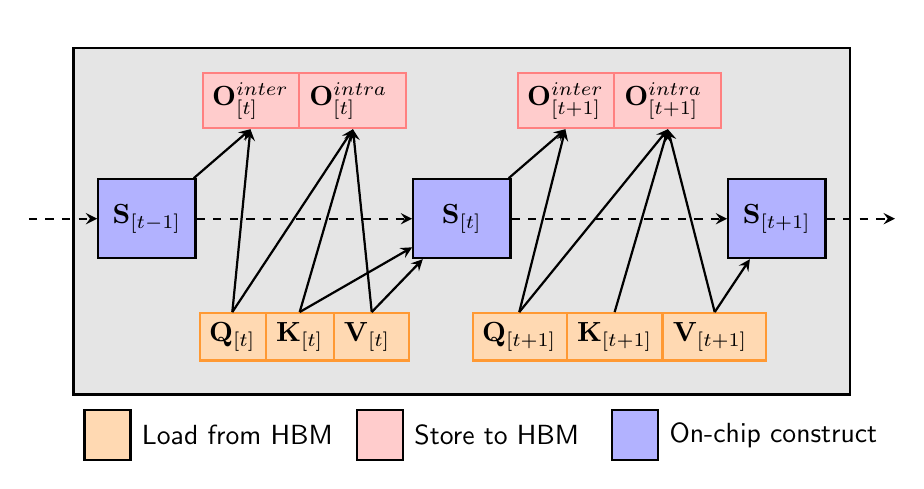
\begin{tikzpicture}[%
            every path/.style={thick,% shorten >=pt, shorten <=2pt
            },
                           dcs/.style = {double copy shadow, shadow xshift=4pt, shadow yshift=-4pt}
          ]
        \node [rectangle, minimum width=.5cm, minimum height=1cm, text centered, text width=1cm,  draw=black, fill=blue!30] (process3) at (-2, -1.5) {$\mathbf{S}_{[t-1]}$};
        
        \node [rectangle, minimum width=.5cm, minimum height=1cm, text centered, text width=1cm,  draw=black, fill=blue!30] (h2) at (2, -1.5) {$\mathbf{S}_{[t]}$};
        \node [rectangle, minimum width=.5cm, minimum height=1cm, text centered, text width=1cm,  draw=black, fill=blue!30] (h3) at (6, -1.5) {$\mathbf{S}_{[t+1]}$};
        
        \node[draw, align=center, draw=red!50, fill=red!20, rectangle split, 
        rectangle split horizontal,
        rectangle split parts=2] (block4) at (4, 0){
        \nodepart{one} $\mathbf{O}^{\text{inter}}_{[t+1]}$ \nodepart{two} $\mathbf{O}^{\text{intra}}_{[t+1]}$ };

    \node[draw,
        align=center,
        draw=red!50,
        fill=red!20,
        rectangle split, 
        rectangle split horizontal,
        rectangle split parts=2] (block2) at (0,0)
    {
        \nodepart{one} $\mathbf{O}^{\text{inter}}_{[t]}$ \nodepart{two} $\mathbf{O}^{\text{intra}}_{[t]}$
    };
    
    \node[BLOCK=3, fill=orange!30, draw=orange!80] (block) at (0,-3) {
        \nodepart{one} $\mathbf{Q}_{[t]}$ \nodepart{two} $\mathbf{K}_{[t]}$ \nodepart{three} $\mathbf{V}_{[t]}$
    };

    \node[BLOCK=3, fill=orange!30, draw=orange!80] (block3) at (4,-3) {
        \nodepart{one} $\mathbf{Q}_{[t+1]}$ \nodepart{two} $\mathbf{K}_{[t+1]}$ \nodepart{three} $\mathbf{V}_{[t+1]}$
    };

    \node [rectangle, text centered, text width=.35cm, text height=.4cm, draw=black, fill=orange!30, label=right:{Load from HBM}] (node1) at (-2.5, -4.25){};
    \node [rectangle, text centered, text width=.35cm, text height=.4cm, draw=black, fill=red!20, label=right:Store to HBM] (node2) at (.96, -4.25){};
    \node [] (labell) at (6, -3.3){};
    \node [rectangle, text centered, text width=.35cm, text height=.4cm, draw=black, fill=blue!30, label=right:On-chip construct] (node3) at (4.2, -4.25){};

    \draw [arrow] (process3) -- (block2.one south);
    \draw [arrow] (h2) -- (block4.one south);
    \draw [arrow] (block.one north) -- (block2.one south);
    \draw [arrow, dashed] (process3) -- (h2);
    \draw [arrow, dashed] (h2) -- (h3);
    \draw [arrow] (block.one north) -- (block2.two south);
    \draw [arrow] (block3.one north) -- (block4.one south);
    \draw [arrow] (block3.two north) -- (block4.two south);
    \draw [arrow] (block3.three north) -- (block4.two south);
    \draw [arrow] (block3.three north) -- (h3);
    \draw [arrow] (block3.one north) -- (block4.two south);
    \draw [arrow] (block.two north) -- (block2.two south);
    \draw [arrow] (block.three north) -- (block2.two south);
    \draw [arrow] (block.two north) -- (h2);
    \draw [arrow] (block.three north) -- (h2);
    \draw [arrow, dashed] ($(process3)-(1.5,0)$) -- (process3);
    \draw [arrow, dashed] (h3) -- ($(h3)+(1.5,0)$);


    \begin{scope}[on background layer]
        \node  [container1,fit= {(process3) (h2) (block) (block2) (h3) (block3) (labell)}, label=north:\large] (contain1) {};
    \end{scope}
        \end{tikzpicture}   
}
        \vspace{-2mm}
        % \caption{(a) \textsc{FlashLinearAttention} without materialization. This version is more memory-efficient.} \label{fig:chunk}
              
    \end{figure}